% !TEX root = ../main.tex
% Хавсралт Г

\chapter{Сегментчлэлийн үр дүнгийн жишээ}
\label{AppendixD}
\pagecolor{white}

Сегментчлэлийн үр дүнгээс харахад ихэнх тохиолдолд хугарлын бүсийг зөв тодорхойлж чадсан боловч жижиг хэмжээтэй болон бүдэг хугарлууд дээр нарийвчлал буурах хандлага ажиглагдсан. Зураг~\ref{fig:appD_more}-д Туршилт 3-ын анхны зураг, ground truth маск болон загварын таамаглалыг (Original / Ground Truth / Prediction) харьцуулсан жишээнүүдийг үзүүлэв.

\begin{figure}[H]
    \centering
    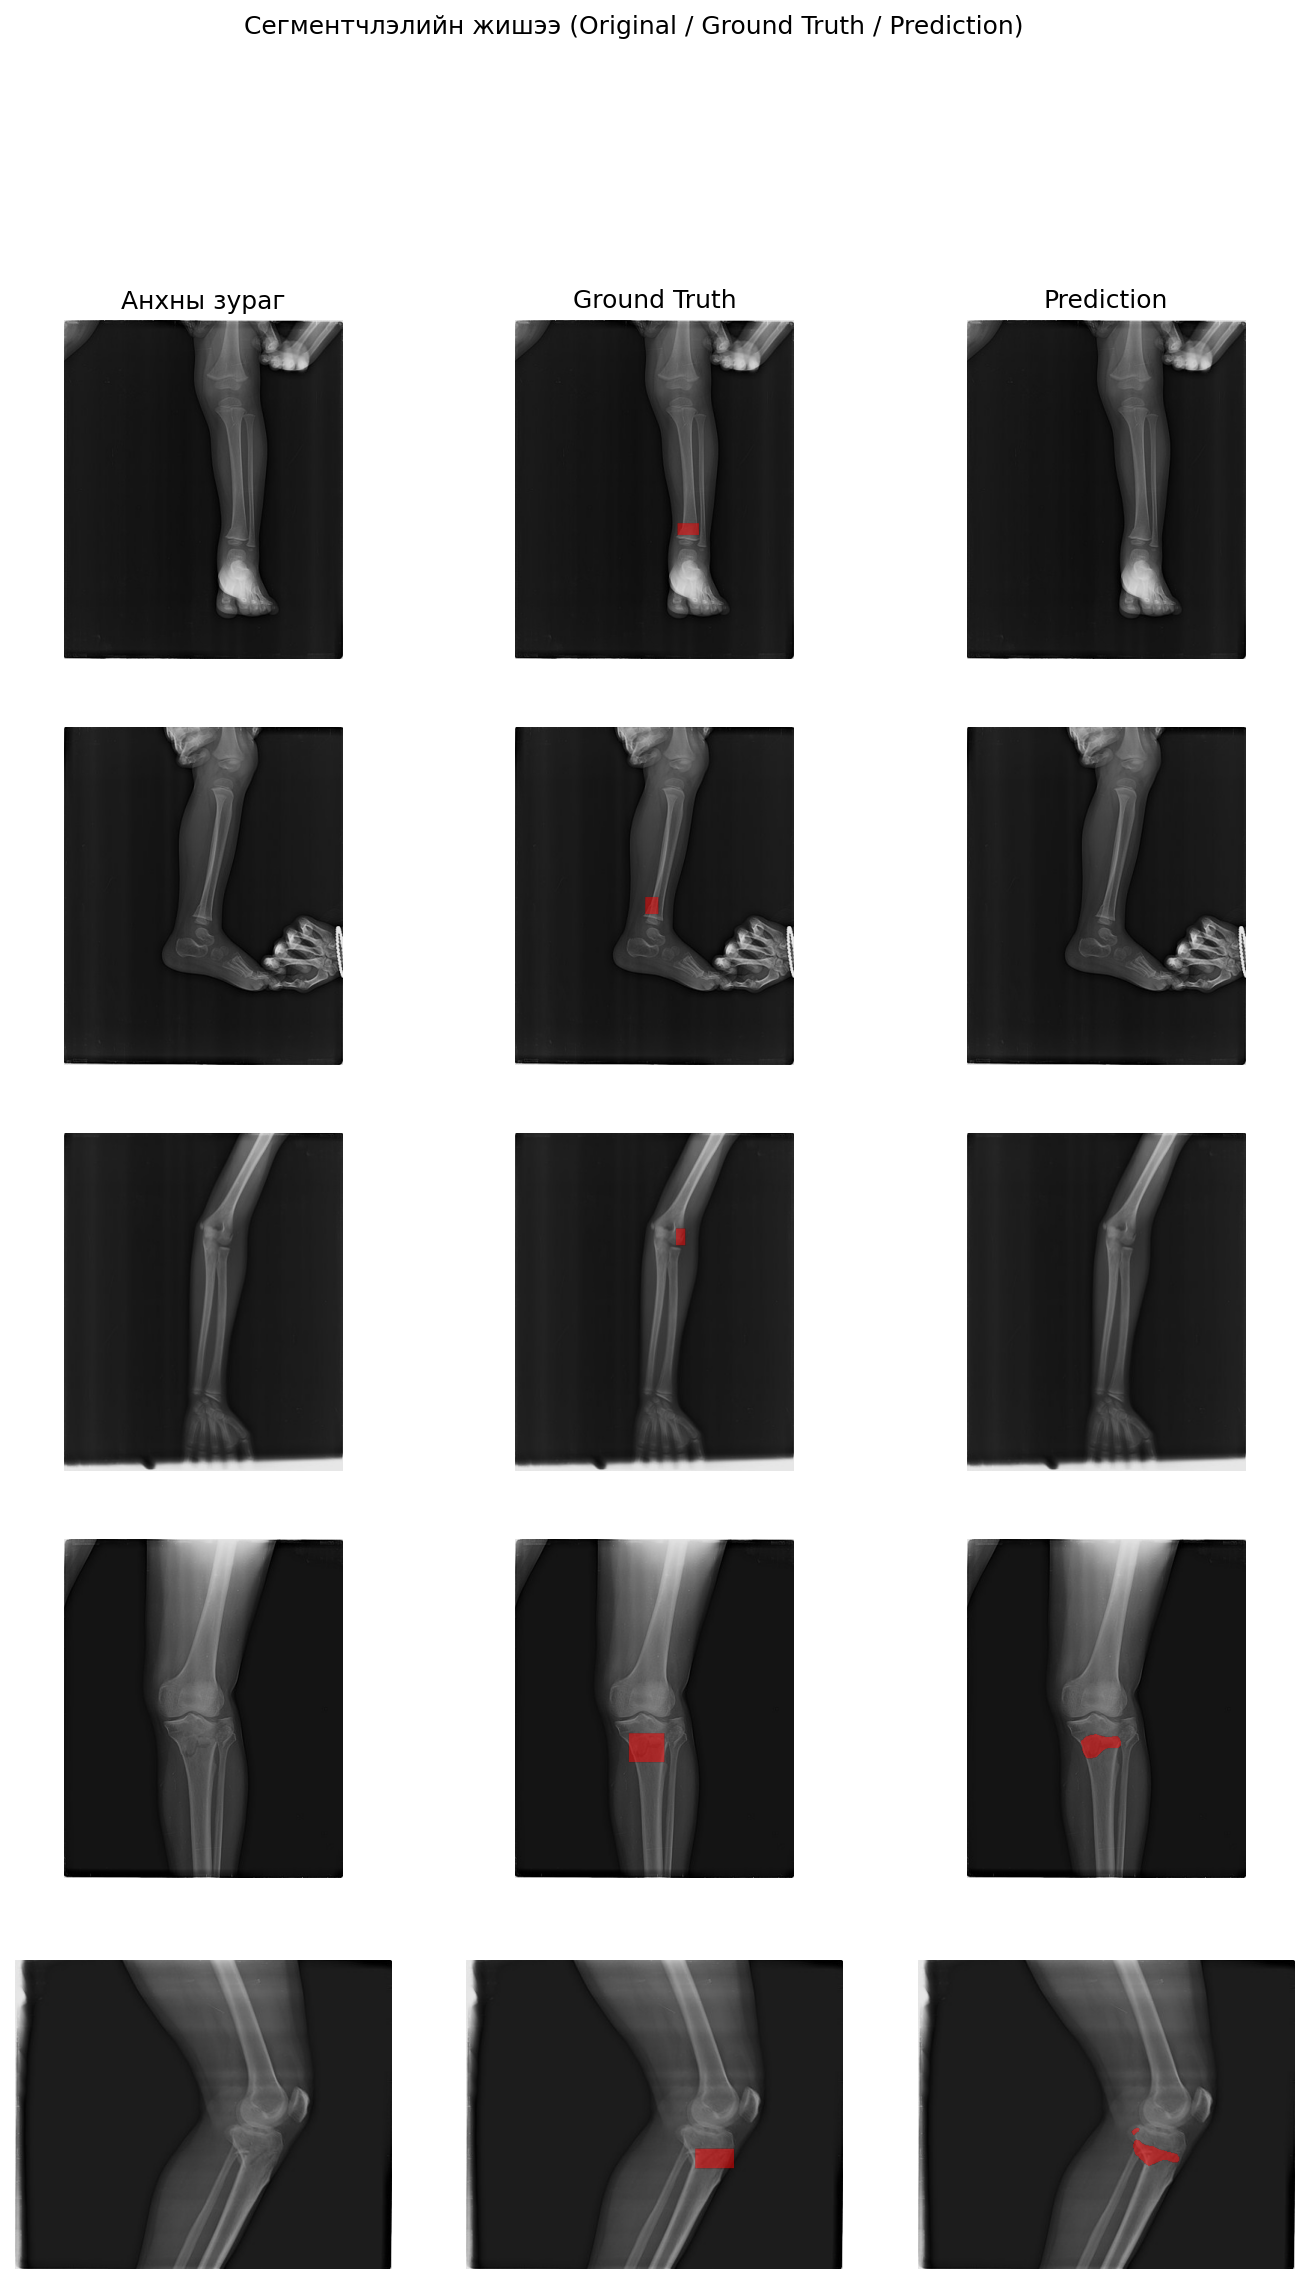
\includegraphics[width=0.78\textwidth,height=0.68\textheight,keepaspectratio]{Figures/appx_d3_seg_triplets.png}
    \figcaption{Нэмэлт сегментчлэлийн жишээнүүд}{Нэмэлт сегментчлэлийн жишээнүүд (\texttt{gen\_D\_segmentation.py})}
    \label{fig:appD_more}
\end{figure}
